\documentclass[../thesis.tex]{subfiles}

\begin{document}

\appendix

\chapter{Data Description}
\label{chap:data_desc}

\noindent In this appendix we present a descriptive overview of the data used in this thesis. This includes: an overview and explanation of the variables used (\ref{sec:variables}), the \texttt{R}-packages (\ref{sec:r_pack}) used and some relevant plots (\ref{sec:rel_plots}) to support the finding in the thesis. The source code used to produce the relevant plots can be found in appendix (\ref{chap:souce_code}).  

\section{Variables}
\label{sec:variables}

\begin{longtable}{p{.22\textwidth}  p{.71\textwidth}}
    \caption{Phenotype domains used for clinical metrics}\vspace*{-0,1cm} \label{tab:var}\\
    \toprule
    \textbf{Phenotype domain} & \textbf{Clinical Variables}\\
    \midrule
\endfirsthead
    \caption*{\textbf{Table \ref{tab:var} Continued:} Phenotype domains used for clinical metrics}\vspace*{-0,1cm}\\
    \toprule
    \textbf{Phenotype domain} & \textbf{Clinical Variables}\\
    \midrule
\endhead
&\\
Demographics & Age, gender, ethnicity\\
&\\
Admission symptoms & Breathless, chest pain, orthnopea, paroxysmal nocturnal dyspnoea, peripheral oedema, palpitations, syncope\\
&\\
Admission signs & Admission heart rate (HR), admission systolic blood pressure (SBP), admission diastolic blood pressure (DBP), admission mean blood pressure (MAP), admission weight, height, admission body mass index, discharge weight\\
&\\
Risk factors & Atrial fibrillation, hypertension, diabetes, chronic obstructive pulmonary disease, coronary artery disease, history of cerebrovascular disease, hypercholesterolaemia, obstructive sleep apnoea, iron deficiency, obesity\\
&\\
Comorbidities & Depression, dementia, amyloidosis, cancer\\
&\\
12 lead electrocardiogram (ECG) & Rhythm, rate, QRS duration, evidence of atrioventricular (AV) block, T wave inversion (TWI), evidence of left ventricular hypertrophy (LVH), presence of pacemaker\\
&\\
Laboratory tests & Haemoglobin, mean cell volume (MCV), packed cell volume (PCV), white blood cells (WBC), platelets, sodium, potassium, glomerular filtration rate (GFR), albumin, HbA1C, glucose, iron levels, transferrin saturations (TSAT), ferritin, troponin\\
&\\
Echocardiography & Left ventricular ejection fraction (LVEF), left atrial diameter left atrial area, right atrial area, E wave, E deceleration time, Lateral e’, lateral S, E/e’, dilated LV, A wave, E:A, gradient, regional wall motion abnormalities, left ventricular hypertrophy, tricuspid annular planesystolic excursion (TAPSE), pulmonary artery systolic pressure (PASP), mitral regurgitation, tricuspid regurgitation, aortic regurgitation, aortic stenosis\\
&\\
Outcome & Length of stay, time to heart failure hospitalization, time to mortality\\
&\\
\midrule
\end{longtable}

\section{\texttt{R}-packages}
\label{sec:r_pack}

\begin{small}
\begin{tabularx}{\textwidth}{lLr}
\caption{Packages used in thesis}\label{tab:packages}\\
\toprule
\textbf{Package} & \textbf{Title} & \textbf{Version}\\
\midrule
\endfirsthead
\caption*{\textbf{Table \ref{tab:packages}:} Packages used in thesis (\textit{continued})}\\
\toprule
\textbf{Package} & \textbf{Title} & \textbf{Version}\\
\midrule
\endhead
Amelia & A Program for Missing Data & 1.7.5 \\ 
BaylorEdPsych & R Package for Baylor University Educational Psychology
Quantitative Courses & 0.5 \\ 
caret & Classification and Regression Training & 6.0-80 \\ 
CBCgrps & Compare Baseline Characteristics Between Groups & 2.3 \\ 
docstring & Provides Docstring Capabilities to R Functions & 1.0.0 \\ 
factoextra & Extract and Visualize the Results of Multivariate Data Analyses & 1.0.5 \\ 
FactoMineR & Multivariate Exploratory Data Analysis and Data Mining & 1.41 \\ 
ggpubr & 'ggplot2' Based Publication Ready Plots & 0.1.8 \\ 
gridExtra & Miscellaneous Functions for "Grid" Graphics & 2.3 \\ 
Hmisc & Harrell Miscellaneous & 4.1-1 \\ 
mclust & Gaussian Mixture Modelling for Model-Based Clustering,
Classification, and Density Estimation & 5.4.1 \\ 
mice & Multivariate Imputation by Chained Equations & 3.3.0 \\ 
mlbench & Machine Learning Benchmark Problems & 2.1-1 \\ 
NbClust & Determining the Best Number of Clusters in a Data Set & 3.0 \\ 
plotrix & Various Plotting Functions & 3.7-4 \\ 
reporttools & Generate LaTeX Tables of Descriptive Statistics & 1.1.2 \\ 
rlist & A Toolbox for Non-Tabular Data Manipulation & 0.4.6.1 \\ 
tikzDevice & R Graphics Output in LaTeX Format & 0.11 \\ 
VIM & Visualization and Imputation of Missing Values & 4.7.0 \\ 
xtable & Export Tables to LaTeX or HTML & 1.8-2 \\ 
\midrule
\end{tabularx}
\end{small}


\newpage

\section{Descriptive statistics}
\label{sec:desc_stat}


\begin{scriptsize}
\begin{tabularx}{\textwidth}{P{3cm}rrrrrrrrrr}
\caption{Patient characteristics: HFpEF}\label{tab:desc_stat_HFpEF_variables}\\
\toprule
\textbf{Variable} & $n$ & \#Na & Min & Max & $\bar{x}$ & $\widetilde{x}$ & $s$ & $q_1$ & $q_3$ \\ 
\midrule
\endfirsthead
\caption*{\textbf{Table \ref{tab:desc_stat_HFpEF_variables}:} Patient characteristics: HFpEF (\textit{continued})}\\
\toprule
 \textbf{Variable} & $n$ & \#Na & Min & Max & $\bar{x}$ & $\widetilde{x}$ & $s$ & $q_1$ & $q_3$ \\ 
\midrule
\endhead
\multicolumn{10}{c}{PANEL II: Demographics}\\
\midrule
  age & 193 &   0 &  29.0 &   100.8 &   76.3 &   78.9 &   12.1 &  69.5 &   85.4 \\ 
  gender & 193 &   0 &   0.0 &     1.0 &    0.6 &    1.0 &    0.5 &   0.0 &    1.0 \\ 
  white & 193 &   0 &   0.0 &     1.0 &    0.7 &    1.0 &    0.5 &   0.0 &    1.0 \\ 
  asian & 193 &   0 &   0.0 &     1.0 &    0.1 &    0.0 &    0.2 &   0.0 &    0.0 \\ 
  black & 193 &   0 &   0.0 &     1.0 &    0.3 &    0.0 &    0.4 &   0.0 &    1.0 \\
\midrule
\multicolumn{10}{c}{PANEL III: Admission symptoms}\\
\midrule
  breathless & 185 &   8 &   0.0 &     1.0 &    0.8 &    1.0 &    0.4 &   1.0 &    1.0 \\ 
\midrule
\multicolumn{10}{c}{PANEL IV: Admission signs}\\
\midrule
  sbp & 182 &  11 &  55.0 &   242.0 &  146.9 &  145.0 &   31.7 & 125.0 &  167.0 \\ 
  dbp & 183 &  10 &  25.0 &   195.0 &   80.5 &   80.0 &   22.1 &  67.0 &   89.0 \\ 
  admissionwgt & 160 &  33 &  41.5 &   158.0 &   78.9 &   76.7 &   23.3 &  60.1 &   93.9 \\ 
  bp & 192 &   1 &   0.0 &     1.0 &    0.8 &    1.0 &    0.4 &   1.0 &    1.0 \\ 
  bmiadmission & 148 &  45 &  16.8 &   107.1 &   30.7 &   29.3 &   10.5 &  23.6 &   35.4 \\ 
  pulse & 182 &  11 &  44.0 &   211.0 &   84.7 &   83.0 &   22.1 &  70.0 &   95.0 \\
\midrule
\multicolumn{10}{c}{PANEL V: Risk factors}\\
\midrule
  a-fib & 189 &   4 &   0.0 &     1.0 &    0.5 &    0.0 &    0.5 &   0.0 &    1.0 \\ 
  copdasthma & 190 &   3 &   0.0 &     1.0 &    0.4 &    0.0 &    0.5 &   0.0 &    1.0 \\ 
  irondef &  69 & 124 &   0.0 &     1.0 &    0.6 &    1.0 &    0.5 &   0.0 &    1.0 \\ 
  dm & 188 &   5 &   0.0 &     1.0 &    0.5 &    1.0 &    0.5 &   0.0 &    1.0 \\ 
  obesity & 185 &   8 &   0.0 &     1.0 &    0.5 &    1.0 &    0.5 &   0.0 &    1.0 \\ 
  copdasthma.1 & 190 &   3 &   0.0 &     1.0 &    0.4 &    0.0 &    0.5 &   0.0 &    1.0 \\ 
  ihd & 186 &   7 &   0.0 &     1.0 &    0.4 &    0.0 &    0.5 &   0.0 &    1.0 \\ 
\midrule
\multicolumn{10}{c}{PANEL VI: Comorbidities}\\
\midrule
  comorbidities & 193 &   0 &   0.0 &     9.0 &    4.2 &    4.0 &    1.8 &   3.0 &    5.0 \\ 
\midrule
\multicolumn{10}{c}{PANEL VII: Electrocardiography}\\
\midrule
  ecgqrsduration & 157 &  36 &  55.0 &   177.0 &  101.3 &   98.0 &   20.8 &  88.0 &  112.0 \\ 
  ecgqrsother & 193 &   0 &   0.0 &     1.0 &    0.0 &    0.0 &    0.2 &   0.0 &    0.0 \\ 
  ecgrate & 159 &  34 &  41.0 &   191.0 &   83.0 &   80.0 &   23.1 &  70.0 &   92.0 \\ 
  ecgrhythmother & 193 &   0 &   0.0 &     1.0 &    0.1 &    0.0 &    0.2 &   0.0 &    0.0 \\ 
  lvh & 169 &  24 &   0.0 &     1.0 &    0.1 &    0.0 &    0.3 &   0.0 &    0.0 \\ 
  normalecgqrs & 193 &   0 &   0.0 &     1.0 &    0.6 &    1.0 &    0.5 &   0.0 &    1.0 \\ 
  lbbb & 193 &   0 &   0.0 &     1.0 &    0.0 &    0.0 &    0.2 &   0.0 &    0.0 \\ 
  rbbb & 193 &   0 &   0.0 &     1.0 &    0.1 &    0.0 &    0.3 &   0.0 &    0.0 \\ 
  sr & 193 &   0 &   0.0 &     1.0 &    0.6 &    1.0 &    0.5 &   0.0 &    1.0 \\
\midrule
\multicolumn{10}{c}{PANEL VIII: Laboratory tests}\\
\midrule
  hb & 192 &   1 &  47.0 &   185.0 &  107.6 &  107.5 &   21.1 &  91.8 &  123.0 \\ 
  wbc & 192 &   1 &   2.9 &   209.4 &   10.2 &    7.6 &   15.8 &   6.0 &   10.5 \\ 
  tsat &  94 &  99 &   4.0 &    92.0 &   20.4 &   18.0 &   13.8 &  11.0 &   24.8 \\ 
  plts & 192 &   1 &  51.0 &   497.0 &  229.4 &  217.0 &   89.5 & 163.0 &  284.2 \\ 
  pcv & 193 &   0 &   0.2 &     0.6 &    0.3 &    0.3 &    0.1 &   0.3 &    0.4 \\ 
  ferritin &  71 & 122 &   9.0 &  2223.0 &  378.2 &  173.0 &  533.8 &  61.5 &  443.5 \\ 
  k & 189 &   4 &   2.4 &     8.7 &    4.4 &    4.4 &    0.6 &   4.1 &    4.7 \\ 
  ironlevels &  95 &  98 &   2.0 &    23.0 &    8.6 &    7.0 &    4.8 &   5.0 &   11.0 \\ 
  chol & 190 &   3 &   0.0 &     1.0 &    0.5 &    1.0 &    0.5 &   0.0 &    1.0 \\ 
  ntprobnp & 193 &   0 &  81.0 & 70000.0 & 5047.3 & 2217.0 & 8487.4 & 997.0 & 5305.0 \\ 
  gfr & 193 &   0 &   3.0 &   221.0 &   54.1 &   47.0 &   31.1 &  32.0 &   72.0 \\ 
  mcv & 193 &   0 &  57.0 &   117.0 &   88.8 &   89.0 &    8.9 &  85.0 &   94.0 \\ 
  na & 193 &   0 & 110.0 &   148.0 &  138.2 &  139.0 &    4.9 & 136.0 &  141.0 \\
\midrule
\multicolumn{10}{c}{PANEL IX: Echocardiography}\\
\midrule
  lvef & 191 &   2 &  50.0 &    72.5 &   57.1 &   57.5 &    4.5 &  55.0 &   60.0 \\ 
  ewave & 174 &  19 &   0.4 &     1.6 &    0.9 &    0.9 &    0.3 &   0.7 &    1.1 \\ 
  pasp & 122 &  71 &  14.0 &    85.0 &   43.5 &   42.5 &   14.2 &  34.0 &   51.8 \\ 
  ee & 152 &  41 &   2.0 &    37.0 &   13.4 &   12.5 &    5.8 &   9.0 &   16.0 \\ 
  mr & 193 &   0 &   0.0 &     2.0 &    0.5 &    0.0 &    0.7 &   0.0 &    1.0 \\ 
  tr & 193 &   0 &   0.0 &     3.0 &    0.9 &    1.0 &    0.8 &   0.0 &    1.0 \\ 
  as & 193 &   0 &   0.0 &     2.0 &    0.1 &    0.0 &    0.3 &   0.0 &    0.0 \\ 
  ai & 193 &   0 &   0.0 &     2.0 &    0.2 &    0.0 &    0.5 &   0.0 &    0.0 \\ 
  rvfunction & 192 &   1 &   0.0 &     4.0 &    0.6 &    0.0 &    1.2 &   0.0 &    0.2 \\ 
  af & 193 &   0 &   0.0 &     1.0 &    0.2 &    0.0 &    0.4 &   0.0 &    0.0 \\ 
\midrule
\multicolumn{10}{c}{PANEL X: Outcomes}\\
\midrule
  timetohfadm &  69 & 124 &   3.8 &   718.8 &  192.5 &  122.7 &  197.8 &  33.0 &  270.0 \\ 
  hfhospitalisation & 193 &   0 &   0.0 &     1.0 &    0.4 &    0.0 &    0.5 &   0.0 &    1.0 \\ 
  los & 171 &  22 &   1.0 &   372.0 &   15.8 &    8.0 &   31.3 &   4.0 &   19.0 \\ 
\midrule
\end{tabularx}
\end{scriptsize}


\begin{scriptsize}
\begin{tabularx}{\textwidth}{P{3cm}RRRRRRRRRR}
\caption{Patient characteristics: HFmrEF}\label{tab:desc_stat_HFmrEF_variables}\\
\toprule
\textbf{Variable}\parnote{\scriptsize Note: $n$ - number of observations, \#Na - number of missing data, Min - minimal, Max - maximal,  $\bar{x}$ - arithmetic mean, $\widetilde{x}$ - median, $s$ - standard deviation, $q_1$ - first quartile and $q_3$ - third quartile.} & $n$ & \# Na & Min & Max & $\bar{x}$ & $\widetilde{x}$ & $s$ & $q_1$ & $q_3$ \\ 
\midrule
\endfirsthead
\caption*{\textbf{Table \ref{tab:desc_stat_HFmrEF_variables}:} Patient characteristics: HFmrEF (\textit{continued})}\\
\toprule
 \textbf{Variable} & $n$ & \#Na & Min & Max & $\bar{x}$ & $\widetilde{x}$ & $s$ & $q_1$ & $q_3$ \\ 
\midrule
\endhead
\multicolumn{10}{c}{PANEL I: Identification}\\
\midrule
patientid & 182 &   0 &     1.0 &    193.0 &    96.9 &    97.5 &    56.6 &    47.2 &   146.5 \\ 
\midrule
\multicolumn{10}{c}{PANEL II: Demographics}\\
\midrule
  gender & 182 &   0 &  0.0 &      1.0 &    0.4 &    0.0 &     0.5 &    0.0 &    1.0 \\ 
  white & 182 &   0 &  0.0 &      1.0 &    0.7 &    1.0 &     0.5 &    0.0 &    1.0 \\ 
  asian & 182 &   0 &  0.0 &      1.0 &    0.1 &    0.0 &     0.3 &    0.0 &    0.0 \\ 
  black & 182 &   0 &  0.0 &      1.0 &    0.2 &    0.0 &     0.4 &    0.0 &    0.0 \\
\midrule
\multicolumn{10}{c}{PANEL III: Admission symptoms}\\
\midrule
  breathless &  55 & 127 &  0.0 &      3.0 &    2.4 &    3.0 &     1.0 &    2.0 &    3.0 \\  
\midrule
\multicolumn{10}{c}{PANEL IV: Admission signs}\\
\midrule
  sbp &  98 &  84 & 86.0 &    242.0 &  132.6 &  126.5 &    27.7 &  114.2 &  147.8 \\ 
  dbp &  95 &  87 & 45.0 &    591.0 &   80.2 &   72.0 &    55.7 &   62.0 &   85.0 \\ 
  admissionwgt &  51 & 131 & 21.0 &    134.9 &   80.6 &   80.6 &    21.8 &   66.7 &   96.4 \\ 
  bp & 182 &   0 &  0.0 &      1.0 &    0.7 &    1.0 &     0.5 &    0.0 &    1.0 \\ 
  bmiadmission &   4 & 178 & 18.7 &     36.1 &   26.0 &   24.7 &     8.0 &   20.2 &   30.5 \\ 
  pulse &  98 &  84 & 54.0 &    144.0 &   88.8 &   85.0 &    21.9 &   71.2 &  100.0 \\
\midrule
\multicolumn{10}{c}{PANEL V: Risk factors}\\
\midrule
  a-fib & 182 &   0 &  0.0 &      1.0 &    0.4 &    0.0 &     0.5 &    0.0 &    1.0 \\ 
  copdasthma & 181 &   1 &  0.0 &      1.0 &    0.3 &    0.0 &     0.5 &    0.0 &    1.0 \\ 
  irondef &  52 & 130 &  0.0 &      1.0 &    0.4 &    0.0 &     0.5 &    0.0 &    1.0 \\ 
  dm & 180 &   2 &  0.0 &      1.0 &    0.4 &    0.0 &     0.5 &    0.0 &    1.0 \\ 
  obesity &  53 & 129 &  0.0 &      1.0 &    0.5 &    1.0 &     0.5 &    0.0 &    1.0 \\ 
  ihd & 181 &   1 &  0.0 &      1.0 &    0.5 &    0.0 &     0.5 &    0.0 &    1.0 \\ 
\midrule
\multicolumn{10}{c}{PANEL VI: Comorbidities}\\
\midrule
  comorbidities & 182 &   0 &  0.0 &      7.0 &    3.2 &    3.0 &     1.7 &    2.0 &    4.0 \\ 
\midrule
\multicolumn{10}{c}{PANEL VII: Electrocardiography}\\
\midrule
  ecgqrsduration &  77 & 105 & 71.0 &    182.0 &  104.9 &   99.0 &    24.0 &   88.0 &  116.0 \\ 
  ecgqrsother & 182 &   0 &  0.0 &      1.0 &    0.1 &    0.0 &     0.2 &    0.0 &    0.0 \\ 
  ecgrate &  88 &  94 & 42.0 &    135.0 &   86.2 &   83.5 &    21.5 &   72.2 &   99.2 \\ 
  ecgrhythmother & 182 &   0 &  0.0 &      1.0 &    0.0 &    0.0 &     0.1 &    0.0 &    0.0 \\ 
  lvh & 180 &   2 &  0.0 &      3.0 &    0.6 &    0.0 &     0.8 &    0.0 &    1.0 \\ 
  normalecgqrs & 182 &   0 &  0.0 &      1.0 &    0.3 &    0.0 &     0.4 &    0.0 &    1.0 \\ 
  lbbb & 182 &   0 &  0.0 &      1.0 &    0.0 &    0.0 &     0.2 &    0.0 &    0.0 \\ 
  rbbb & 182 &   0 &  0.0 &      1.0 &    0.0 &    0.0 &     0.2 &    0.0 &    0.0 \\ 
  sr & 182 &   0 &  0.0 &      1.0 &    0.0 &    0.0 &     0.2 &    0.0 &    0.0 \\
\midrule
\multicolumn{10}{c}{PANEL VIII: Laboratory tests}\\
\midrule
  hb & 168 &  14 & 54.0 &    153.0 &  110.7 &  111.0 &    19.9 &   98.0 &  125.0 \\ 
  wbc & 166 &  16 &  1.5 &     39.2 &    8.3 &    7.6 &     4.2 &    5.9 &    9.4 \\ 
  tsat &  71 & 111 &  1.0 &     65.0 &   20.4 &   19.0 &    12.5 &   14.0 &   25.0 \\ 
  plts & 166 &  16 & 55.0 &    638.0 &  203.8 &  187.0 &    92.3 &  143.2 &  246.5 \\ 
  pcv & 166 &  16 &  0.2 &      0.5 &    0.3 &    0.3 &     0.1 &    0.3 &    0.4 \\ 
  ferritin &  54 & 128 & 17.0 &   3853.0 &  370.2 &  225.0 &   556.3 &  102.8 &  448.0 \\ 
  k & 165 &  17 &  3.0 &      6.1 &    4.4 &    4.4 &     0.6 &    4.0 &    4.8 \\ 
  ironlevels &  70 & 112 &  2.0 &     41.0 &    9.5 &    8.0 &     7.1 &    5.0 &   11.0 \\ 
  chol & 181 &   1 &  0.0 &      1.0 &    0.4 &    0.0 &     0.5 &    0.0 &    1.0 \\ 
  ntprobnp & 182 &   0 &  5.0 &  70000.0 & 9604.4 & 4063.5 & 14051.2 & 1886.5 & 9968.2 \\ 
  gfr & 167 &  15 &  3.0 &    400.0 &   53.5 &   47.0 &    39.8 &   31.0 &   68.5 \\ 
  mcv & 166 &  16 & 65.0 &    112.0 &   91.0 &   92.0 &     8.4 &   86.0 &   96.0 \\ 
  na & 168 &  14 &  4.7 &    155.0 &  137.5 &  139.0 &    11.5 &  136.0 &  141.0 \\
\midrule
\multicolumn{10}{c}{PANEL IX: Echocardiography}\\
\midrule
  lvef & 182 &   0 & 40.0 &     50.0 &   44.0 &   45.0 &     2.9 &   42.0 &   47.5 \\ 
  ewave & 139 &  43 &  0.3 &      5.0 &    0.9 &    0.9 &     0.5 &    0.7 &    1.0 \\ 
  pasp &  72 & 110 & 18.0 & 251520.0 & 3856.5 &   40.0 & 29625.6 &   32.0 &   53.2 \\ 
  ee &  88 &  94 &  3.0 &     43.0 &   14.9 &   13.5 &     7.3 &    9.0 &   19.2 \\ 
  mr & 159 &  23 &  0.0 &      3.0 &    0.8 &    1.0 &     0.8 &    0.0 &    1.0 \\ 
  tr & 157 &  25 &  0.0 &      3.0 &    0.9 &    1.0 &     0.9 &    0.0 &    1.0 \\ 
  as & 140 &  42 &  0.0 &      2.0 &    0.2 &    0.0 &     0.5 &    0.0 &    0.0 \\ 
  ai & 151 &  31 &  0.0 &      3.0 &    0.3 &    0.0 &     0.5 &    0.0 &    0.0 \\ 
  rvfunction & 146 &  36 &  0.0 &      6.0 &    1.2 &    0.0 &     2.0 &    0.0 &    1.0 \\ 
  af & 182 &   0 &  0.0 &      1.0 &    0.2 &    0.0 &     0.4 &    0.0 &    0.0 \\ 
\midrule
\multicolumn{10}{c}{PANEL X: Outcomes}\\
\midrule
  timetohfadm & 122 &  60 &  0.4 &    575.9 &   84.5 &   44.9 &   109.6 &   11.9 &  114.7 \\ 
  hfhospitalisation & 182 &   0 &  0.0 &      1.0 &    0.2 &    0.0 &     0.4 &    0.0 &    0.0 \\ 
  los & 169 &  13 &  1.0 &    196.0 &   16.9 &    9.0 &    24.2 &    4.0 &   19.0 \\ 
\midrule
\end{tabularx}
\vspace*{-0,5cm}\parnotes
\end{scriptsize}

\newpage

\begin{footnotesize}
\begin{tabularx}{1.2\textwidth}{LLLLp{1.7cm}p{3cm}}
\caption{Baseline characteristics of Hierarchical clustering HFpEF based on post-diagnosis}\label{tab:baseline_char_phy_p_hc}\\
\toprule
& Cluster1 & Cluster2 & Cluster3 & $p$-value\\
\midrule
\endfirsthead
\caption*{\textbf{Table \ref{tab:baseline_char_phy_p_hc}:} Baseline characteristics of Hierarchical clustering HFpEF based on post-diagnosis (\textit{continued})}\\
\toprule
& Cluster1 & Cluster2 & Cluster3 & $p$-value\\
\midrule
\endhead
hb & 89.62±15.25 & 107.37±15.78 & 120.22±19.61 & 0.000*** \\ 
pcv & 0.28±0.05 & 0.33±0.05 & 0.37±0.06 & 0.000*** \\ 
age & 77.07(64.44,81.8) & 85.45(77.81,88.81) & 75.27(67.08,82.06) & 0.000*** \\ 
dbp & 75(65,84) & 80(67.25,85.65) & 84(69.5,92) & 0.053 \\ 
ewave & 1.02(0.9,1.2) & 0.9(0.77,1) & 0.9(0.7,1) & 0.000*** \\ 
gfr & 31(22.75,45) & 47(38.25,70.75) & 60(41,84) & 0.000*** \\ 
k & 4.45(4.17,4.8) & 4.2(3.7,4.6) & 4.4(4.1,4.7) & 0.030** \\ 
los & 11(5,21.29) & 10.5(5,22.18) & 7(4,20.87) & 0.217 \\ 
lvef & 57.5(55,60) & 55.5(52.5,57.5) & 57.5(55,60) & 0.063 \\ 
mcv & 87(80.75,92) & 90(85.25,95) & 90(86,95.5) & 0.010** \\ 
na & 138(134.75,141) & 139(137,142) & 139(137,141) & 0.107 \\ 
ntprobnp & 2745(1622,7647.25) & 2432(1269.75,5920.5) & 1417(714.5,3601.5) & 0.001*** \\
plts & 244.5(170,307.25) & 212(164,247) & 215(162,286.5) & 0.393 \\ 
pulse & 82(69.75,92.75) & 79.5(66.75,89.5) & 88(71.5,97.5) & 0.105 \\ 
sbp & 157(128.75,180) & 144.5(129.25,153.94) & 147(124.5,164.5) & 0.200 \\ 
wbc & 7.65(5.37,10.35) & 7.15(5.72,10.7) & 8.1(6.45,10.3) & 0.270 \\ 
\midrule
\multicolumn{3}{l}{Total number of significant baseline char:} & 55\\
\multicolumn{3}{l}{\hspace*{0,5cm} Continuous: } & 8\\
\multicolumn{3}{l}{\hspace*{0,5cm} Categorical: } & 47\\
\midrule
\end{tabularx}
\end{footnotesize}

\newpage

\begin{footnotesize}
\begin{tabularx}{1.2\textwidth}{LLLLp{1.7cm}p{3cm}}
\caption{Baseline characteristics of K-Means clustering HFpEF based on post-diagnosis}\label{tab:baseline_char_phy_p_km}\\
\toprule
& Cluster1 & Cluster2 & Cluster3 & $p$-value\\
\midrule
\endfirsthead
\caption*{\textbf{Table \ref{tab:baseline_char_phy_p_km}:} Baseline characteristics of K-Means clustering HFpEF based on post-diagnosis (\textit{continued})}\\
\toprule
& Cluster1 & Cluster2 & Cluster3 & $p$-value\\
\midrule
\endhead
hb & 120.22±19.61 & 107.37±15.78 & 89.62±15.25 & 0.000*** \\ 
pcv & 0.37±0.06 & 0.33±0.05 & 0.28±0.05 & 0.000*** \\ 
age & 75.27(67.08,82.06) & 85.45(77.81,88.81) & 77.07(64.44,81.8) & 0.000*** \\ 
ewave & 0.9(0.7,1) & 0.9(0.77,1) & 1.02(0.9,1.2) & 0.000*** \\ 
gfr & 60(41,84) & 47(38.25,70.75) & 31(22.75,45) & 0.000*** \\ 
k & 4.4(4.1,4.7) & 4.2(3.7,4.6) & 4.45(4.17,4.8) & 0.030* \\ 
los & 7(4,20.87) & 10.5(5,22.18) & 11(5,21.29) & 0.217 \\ 
lvef & 57.5(55,60) & 55.5(52.5,57.5) & 57.5(55,60) & 0.063 \\ 
mcv & 90(86,95.5) & 90(85.25,95) & 87(80.75,92) & 0.010* \\ 
na & 139(137,141) & 139(137,142) & 138(134.75,141) & 0.107 \\ 
ntprobnp & 1417(714.5,3601.5) & 2432(1269.75,5920.5) & 2745(1622,7647.25) & 0.001** \\ 
plts & 215(162,286.5) & 212(164,247) & 244.5(170,307.25) & 0.393 \\ 
wbc & 8.1(6.45,10.3) & 7.15(5.72,10.7) & 7.65(5.37,10.35) & 0.270 \\ 
\midrule
\multicolumn{3}{l}{Total number of significant baseline char:} & 49\\
\multicolumn{3}{l}{\hspace*{0,5cm} Continuous: } & 8\\
\multicolumn{3}{l}{\hspace*{0,5cm} Categorical: } & 41\\
\midrule
\end{tabularx}
\end{footnotesize}

\newpage

\begin{footnotesize}
\begin{tabularx}{1.2\textwidth}{LLLLp{1.7cm}p{3cm}}
\caption[EM clustering HFpEF based on post-diagnosis]{Baseline characteristics of EM clustering HFpEF based on post-diagnosis}\label{tab:baseline_char_phy_p_em}\\
\toprule
& Cluster1 & Cluster2 & Cluster3 & $p$-value\\
\midrule
\endfirsthead
\caption*{\textbf{Table \ref{tab:baseline_char_phy_p_em}:} Baseline characteristics of EM clustering HFpEF based on post-diagnosis (\textit{continued})}\\
\toprule
& Cluster1 & Cluster2 & Cluster3 & $p$-value\\
\midrule
\endhead
hb & 105.98±17.53 & 89.37±14.55 & 118.61±19.42 & 0.000*** \\ 
pcv & 0.33±0.05 & 0.28±0.04 & 0.37±0.06 & 0.000*** \\ 
age & 85.45(77.81,88.65) & 75(63.26,80.41) & 77.03(68.05,82.11) & 0.000*** \\ 
ewave & 0.9(0.79,1) & 1.1(0.9,1.2) & 0.9(0.7,1) & 0.000*** \\ 
gfr & 45.5(38,67.75) & 31(21.25,45) & 60(40,84) & 0.000*** \\ 
k & 4.2(3.7,4.6) & 4.4(4.13,4.8) & 4.5(4.1,4.7) & 0.012* \\ 
los & 11(5,22.18) & 11.5(4.25,21.76) & 8(4,20.14) & 0.269 \\ 
lvef & 56.75(52.5,57.5) & 57.5(55,60) & 57.5(55,60) & 0.194 \\ 
mcv & 89.5(85.25,94) & 87(80.25,92) & 90(86,97) & 0.008** \\ 
na & 139.5(137,142) & 138(135,141) & 139(136,141) & 0.102 \\ 
ntprobnp & 2755(1451.5,6684.25) & 2745(1566,7993.75) & 1525(727,3590) & 0.000*** \\ 
plts & 212(164,247) & 235.5(170,309.75) & 219(163,284) & 0.402 \\ 
wbc & 7.15(5.8,10.77) & 7.55(5.42,10.17) & 7.9(6.4,10.3) & 0.506 \\
\midrule
\multicolumn{3}{l}{Total number of significant baseline char:} & 56\\
\multicolumn{3}{l}{\hspace*{0,5cm} Continuous: } & 8\\
\multicolumn{3}{l}{\hspace*{0,5cm} Categorical: } & 48\\
\midrule
\end{tabularx}
\end{footnotesize}

\newpage

\begin{footnotesize}
\begin{tabularx}{1.2\textwidth}{LLLLp{1.7cm}p{3cm}}
\caption[Hierarchical clustering HFmrEF based on post-diagnosis]{Baseline characteristics of Hierarchical clustering HFmrEF based on post-diagnosis}\label{tab:baseline_char_phy_mr_hc}\\
\toprule
& Cluster1 & Cluster2 & Cluster3 & $p$-value\\
\midrule
\endfirsthead
\caption*{\textbf{Table \ref{tab:baseline_char_phy_mr_hc}:} Baseline characteristics of Hierarchical clustering HFmrEF based on post-diagnosis (\textit{continued})}\\
\toprule
& Cluster1 & Cluster2 & Cluster3 & $p$-value\\
\midrule
\endhead
hb & 91.01±14.72 & 109.11±16.81 & 123.79±12.89 & 0.000*** \\ 
k & 4.58±0.66 & 4.51±0.58 & 4.18±0.48 & 0.000*** \\ 
pcv & 0.28±0.04 & 0.34±0.05 & 0.38±0.04 & 0.000*** \\ 
age & 71.53(65.87,82.74) & 77.15(70.09,82.04) & 79.19(68.12,82.9) & 0.455 \\ 
ewave & 0.8(0.7,1) & 0.96(0.8,1.14) & 0.83(0.67,0.96) & 0.003** \\ 
gfr & 49.98(22,77) & 43(30,55) & 62(44.5,77.25) & 0.000*** \\ 
los & 17(10,36) & 12(4,21.48) & 7(3,14.25) & 0.000*** \\ 
lvef & 45(42,47.5) & 45(42,47.5) & 42.75(42.5,45) & 0.344 \\ 
mcv & 91(87,96) & 90(85,95) & 93(88,97) & 0.159 \\ 
na & 138(135,141) & 139(135,141) & 139(137.02,142) & 0.049* \\ 
ntprobnp & 6598(2857,27818) & 4953(1861,10914) & 2898.5(1587.75,5163.5) & 0.005** \\ 
plts & 210(147,285) & 204(153,250) & 174.74(149.5,215.75) & 0.107 \\ 
wbc & 8.2(6.3,9.6) & 8.3(6.9,9.8) & 7.31(5.7,8.6) & 0.025 \\ 
\midrule
\multicolumn{3}{l}{Total number of significant baseline char:} & 53\\
\multicolumn{3}{l}{\hspace*{0,5cm} Continuous: } & 8\\
\multicolumn{3}{l}{\hspace*{0,5cm} Categorical: } & 45\\
\midrule
\end{tabularx}
\end{footnotesize}

\newpage

\begin{footnotesize}
\begin{tabularx}{1.2\textwidth}{LLLLp{1.7cm}p{3cm}}
\caption{Baseline characteristics of K-Means clustering HFmrEF based on post-diagnosis}\label{tab:baseline_char_phy_mr_km}\\
\toprule
& Cluster1 & Cluster2 & Cluster3 & $p$-value\\
\midrule
\endfirsthead
\caption*{\textbf{Table \ref{tab:baseline_char_phy_mr_km}:} Baseline characteristics of K-Means clustering HFmrEF based on post-diagnosis (\textit{continued})}\\
\toprule
& Cluster1 & Cluster2 & Cluster3 & $p$-value\\
\midrule
\endhead
hb & 91.01±14.72 & 109.11±16.81 & 123.79±12.89 & 0.000*** \\ 
k & 4.58±0.66 & 4.51±0.58 & 4.18±0.48 & 0.000*** \\ 
pcv & 0.28±0.04 & 0.34±0.05 & 0.38±0.04 & 0.000*** \\ 
age & 71.53(65.87,82.74) & 77.15(70.09,82.04) & 79.19(68.12,82.9) & 0.455 \\ 
ewave & 0.8(0.7,1) & 0.96(0.8,1.14) & 0.83(0.67,0.96) & 0.003** \\ 
gfr & 49.98(22,77) & 43(30,55) & 62(44.5,77.25) & 0.000*** \\ 
los & 17(10,36) & 12(4,21.48) & 7(3,14.25) & 0.000*** \\ 
lvef & 45(42,47.5) & 45(42,47.5) & 42.75(42.5,45) & 0.344 \\ 
mcv & 91(87,96) & 90(85,95) & 93(88,97) & 0.159 \\ 
na & 138(135,141) & 139(135,141) & 139(137.02,142) & 0.049* \\ 
ntprobnp & 6598(2857,27818) & 4953(1861,10914) & 2898.5(1587.75,5163.5) & 0.005** \\ 
plts & 210(147,285) & 204(153,250) & 174.74(149.5,215.75) & 0.107 \\ 
wbc & 8.2(6.3,9.6) & 8.3(6.9,9.8) & 7.31(5.7,8.6) & 0.025 \\ 
\midrule
\multicolumn{3}{l}{Total number of significant baseline char:} & 53\\
\multicolumn{3}{l}{\hspace*{0,5cm} Continuous: } & 8\\
\multicolumn{3}{l}{\hspace*{0,5cm} Categorical: } & 45\\
\midrule
\end{tabularx}
\end{footnotesize}

\newpage

\begin{footnotesize}
\begin{tabularx}{1.2\textwidth}{LLLLp{1.7cm}p{3cm}}
\caption{Baseline characteristics of EM clustering HFmrEF based on post-diagnosis}\label{tab:baseline_char_phy_mr_em}\\
\toprule
& Cluster1 & Cluster2 & Cluster3 & $p$-value\\
\midrule
\endfirsthead
\caption*{\textbf{Table \ref{tab:baseline_char_phy_mr_em}:} Baseline characteristics of EM clustering HFmrEF based on post-diagnosis (\textit{continued})}\\
\toprule
& Cluster1 & Cluster2 & Cluster3 & $p$-value\\
\midrule
\endhead
hb & 83.17±14.19 & 105.83±17.56 & 120.8±14.91 & 0.000*** \\ 
k & 4.65±0.84 & 4.53±0.57 & 4.22±0.51 & 0.001** \\ 
pcv & 0.26±0.04 & 0.33±0.05 & 0.37±0.04 & 0.000*** \\ 
age & 68.63(41.33,74.15) & 76.91(69.62,82.01) & 80.97(68.7,83.32) & 0.031 \\ 
ewave & 0.88(0.7,1.01) & 0.94(0.79,1.12) & 0.82(0.67,0.95) & 0.009** \\ 
gfr & 27(13.75,82.25) & 42.5(27.5,58) & 61(45.75,76.25) & 0.000*** \\ 
los & 27.5(13.75,62) & 12.5(5,21) & 8(3,16.5) & 0.006** \\ 
lvef & 45(42,45.62) & 45(42,47.5) & 43(42.5,45) & 0.517 \\ 
mcv & 91.5(86,96) & 89.94(85.06,94) & 93(89,97) & 0.027* \\ 
na & 136.5(133.75,141) & 139(135.25,141) & 139(137,142) & 0.175 \\ 
ntprobnp & 19446.5(4178.5,59423.25) & 5640.5(1953.25,11400.75) & 2898.5(1636,5163.5) & 0.001** \\ 
plts & 155(117,236.25) & 205.36(157.25,256) & 177.5(147,224) & 0.081 \\ 
wbc & 6.55(5.6,7.77) & 8.4(7.1,10.3) & 7.25(5.7,8.8) & 0.001** \\ 
\midrule
\multicolumn{3}{l}{Total number of significant baseline char:} & 44\\
\multicolumn{3}{l}{\hspace*{0,5cm} Continuous: } & 9\\
\multicolumn{3}{l}{\hspace*{0,5cm} Categorical: } & 35\\
\midrule
\end{tabularx}
\end{footnotesize}

\newpage

\begin{footnotesize}
\begin{tabularx}{1.2\textwidth}{LLLLp{1.7cm}p{3cm}}
\caption{Baseline characteristics of Hierarchical clustering HFpEF without post-diagnosis}\label{tab:baseline_char_nophy_p_hc}\\
\toprule
& Cluster1 & Cluster2 & Cluster3 & $p$-value\\
\midrule
\endfirsthead
\caption*{\textbf{Table \ref{tab:baseline_char_nophy_p_hc}:} Baseline characteristics of Hierarchical clustering HFpEF without post-diagnosis (\textit{continued})}\\
\toprule
& Cluster1 & Cluster2 & Cluster3 & $p$-value\\
\midrule
\endhead
hb & 87.94±13.31 & 110.91±17.01 & 117.31±20.34 & 0.000*** \\ 
pcv & 0.28±0.04 & 0.34±0.05 & 0.37±0.06 & 0.000*** \\ 
age & 75(64.94,81.79) & 84.31(77.36,88.63) & 74.08(65.25,82.89) & 0.000*** \\ 
ewave & 1.1(0.92,1.27) & 0.9(0.7,1) & 0.94(0.7,1.1) & 0.000*** \\ 
gfr & 29(20.5,44.25) & 47(38,68) & 55.5(40.25,83.75) & 0.000*** \\ 
k & 4.44(4.1,4.8) & 4.2(3.7,4.5) & 4.45(3.92,4.78) & 0.008** \\ 
los & 12(5,22.19) & 10(4,23.83) & 8(4,20.76) & 0.246 \\ 
lvef & 55(52.5,58.12) & 57.5(55,60) & 57.5(55,60) & 0.203 \\ 
mcv & 87(79.25,92) & 89(85,94) & 90.5(85.25,96) & 0.039 \\ 
na & 137.5(134.75,141) & 140(137,142) & 139.5(137,141) & 0.024** \\ 
ntprobnp & 3852(1879.5,9806.75) & 1995(934,5573) & 1653.5(870.25,3760.75) & 0.000*** \\ 
plts & 226(162,303.75) & 210(170,251.5) & 217(160.25,296.5) & 0.889 \\ 
wbc & 7.75(5.7,9.92) & 7.2(5.55,10.55) & 8.1(6.63,11.13) & 0.121 \\ 
\midrule
\multicolumn{3}{l}{Total number of significant baseline char:} & 48\\
\multicolumn{3}{l}{\hspace*{0,5cm} Continuous: } & 8\\
\multicolumn{3}{l}{\hspace*{0,5cm} Categorical: } & 40\\
\midrule
\end{tabularx}
\end{footnotesize}

\newpage

\begin{footnotesize}
\begin{tabularx}{1.2\textwidth}{LLLLp{1.7cm}p{3cm}}
\caption{Baseline characteristics of K-Means clustering HFpEF without post-diagnosis}\label{tab:baseline_char_nophy_p_km}\\
\toprule
& Cluster1 & Cluster2 & Cluster3 & $p$-value\\
\midrule
\endfirsthead
\caption*{\textbf{Table \ref{tab:baseline_char_nophy_p_km}:} Baseline characteristics of K-Means clustering HFpEF without post-diagnosis (\textit{continued})}\\
\toprule
& Cluster1 & Cluster2 & Cluster3 & $p$-value\\
\midrule
\endhead
hb & 117.31±20.34 & 87.94±13.31 & 110.91±17.01 & 0.000*** \\ 
pcv & 0.37±0.06 & 0.28±0.04 & 0.34±0.05 & 0.000*** \\ 
age & 74.08(65.25,82.89) & 75(64.94,81.79) & 84.31(77.36,88.63) & 0.000*** \\ 
ewave & 0.94(0.7,1.1) & 1.1(0.92,1.27) & 0.9(0.7,1) & 0.000*** \\ 
gfr & 55.5(40.25,83.75) & 29(20.5,44.25) & 47(38,68) & 0.000*** \\ 
k & 4.45(3.92,4.78) & 4.44(4.1,4.8) & 4.2(3.7,4.5) & 0.008** \\ 
los & 8(4,20.76) & 12(5,22.19) & 10(4,23.83) & 0.246 \\ 
lvef & 57.5(55,60) & 55(52.5,58.12) & 57.5(55,60) & 0.203 \\ 
mcv & 90.5(85.25,96) & 87(79.25,92) & 89(85,94) & 0.039 \\ 
na & 139.5(137,141) & 137.5(134.75,141) & 140(137,142) & 0.024** \\ 
ntprobnp & 1653.5(870.25,3760.75) & 3852(1879.5,9806.75) & 1995(934,5573) & 0.000*** \\ 
plts & 217(160.25,296.5) & 226(162,303.75) & 210(170,251.5) & 0.889 \\ 
wbc & 8.1(6.63,11.13) & 7.75(5.7,9.92) & 7.2(5.55,10.55) & 0.121 \\ 
\midrule
\multicolumn{3}{l}{Total number of significant baseline char:} & 48\\
\multicolumn{3}{l}{\hspace*{0,5cm} Continuous: } & 8\\
\multicolumn{3}{l}{\hspace*{0,5cm} Categorical: } & 40\\
\midrule
\end{tabularx}
\end{footnotesize}

\newpage

\begin{footnotesize}
\begin{tabularx}{1.2\textwidth}{LLLLp{1.7cm}p{3cm}}
\caption{Baseline characteristics of EM clustering HFpEF without post-diagnosis}\label{tab:baseline_char_nophy_p_em}\\
\toprule
& Cluster1 & Cluster2 & Cluster3 & $p$-value\\
\midrule
\endfirsthead
\caption*{\textbf{Table \ref{tab:baseline_char_nophy_p_em}:} Baseline characteristics of EM clustering HFpEF without post-diagnosis (\textit{continued})}\\
\toprule
& Cluster1 & Cluster2 & Cluster3 & $p$-value\\
\midrule
\endhead
hb & 106.38±16.53 & 84.31±14.29 & 109.8±21.75 & 0.000*** \\ 
pcv & 0.33±0.05 & 0.27±0.04 & 0.34±0.07 & 0.000*** \\ 
age & 84.69(76.93,88.61) & 71.3(60.76,82.33) & 77.79(68.05,84.04) & 0.001** \\ 
ewave & 0.9(0.68,1) & 1.1(0.96,1.2) & 0.98(0.8,1.1) & 0.007** \\ 
gfr & 44(36.5,56.5) & 26.5(10,38.5) & 48(31,73) & 0.000*** \\ 
k & 4.1(3.7,4.5) & 4.4(4.17,4.75) & 4.4(4.1,4.7) & 0.024* \\ 
los & 10(4,21.54) & 8.5(4,16.5) & 10(5,22.08) & 0.652 \\ 
lvef & 57.5(54.38,60.62) & 57.5(54.38,60.62) & 57.5(52.5,60) & 0.357 \\ 
mcv & 89(85,93.25) & 89(83,93.25) & 89(84,95) & 0.914 \\ 
na & 140(137,142) & 137(134,141.25) & 139(136,141) & 0.233 \\ 
ntprobnp & 2191.5(1048,5046.25) & 4114.5(1707,10007.75) & 2184(976,4895) & 0.098 \\ 
plts & 206.5(163.75,243.75) & 206.5(154,296.75) & 221(163,301) & 0.494 \\ 
wbc & 7.1(5.5,9.35) & 7.05(4.75,9.1) & 8.1(6.4,10.9) & 0.045* \\ 
\midrule
\multicolumn{3}{l}{Total number of significant baseline char:} & 42\\
\multicolumn{3}{l}{\hspace*{0,5cm} Continuous: } & 6\\
\multicolumn{3}{l}{\hspace*{0,5cm} Categorical: } & 36\\
\midrule
\end{tabularx}
\end{footnotesize}

\newpage

\begin{footnotesize}
\begin{tabularx}{1.2\textwidth}{LLLLp{1.7cm}p{3cm}}
\caption{Baseline characteristics of Hierarchical clustering HFmrEF without post-diagnosis}\label{tab:baseline_char_nophy_mr_hc}\\
\toprule
& Cluster1 & Cluster2 & Cluster3 & $p$-value\\
\midrule
\endfirsthead
\caption*{\textbf{Table \ref{tab:baseline_char_nophy_mr_hc}:} Baseline characteristics of Hierarchical clustering HFmrEF without post-diagnosis (\textit{continued})}\\
\toprule
& Cluster1 & Cluster2 & Cluster3 & $p$-value\\
\midrule
\endhead
hb & 89.5±14.24 & 122.31±13.84 & 113.5±15.95 & 0.000*** \\ 
k & 4.55±0.66 & 4.32±0.49 & 4.46±0.61 & 0.114 \\ 
age & 72.08(67.43,82.83) & 81.14(74.51,85.01) & 77.02(67.73,81.93) & 0.006** \\ 
ewave & 0.8(0.7,1) & 0.82(0.62,0.99) & 0.9(0.8,1.05) & 0.026* \\ 
gfr & 41(21.75,76.25) & 64(47,82.5) & 44(31,60.86) & 0.000*** \\ 
los & 15.5(8.75,34.5) & 9(4,24) & 9(3,18) & 0.003** \\ 
lvef & 45(41.61,47.5) & 45(42.5,47.5) & 42.5(40,47.5) & 0.001*** \\ 
mcv & 91(86,96.25) & 93(88.71,96) & 90(86.75,94) & 0.136 \\ 
na & 138(134.75,141) & 139(136,141) & 139(136.92,141) & 0.663 \\ 
ntprobnp & 8937.5(3303.5,26619.5) & 2898.5(1440.75,5004.5) & 3817.5(1647.25,10311.75) & 0.000*** \\ 
pcv & 0.28(0.26,0.31) & 0.38(0.35,0.4) & 0.36(0.33,0.38) & 0.000*** \\ 
plts & 210.5(151.5,285.5) & 193(148.5,231.5) & 191.27(153.75,226.5) & 0.466 \\ 
wbc & 8.65(6.25,12.45) & 7.45(6.07,9.22) & 8.3(5.87,11.15) & 0.375 \\ 
\midrule
\multicolumn{3}{l}{Total number of significant baseline char:} & 51\\
\multicolumn{3}{l}{\hspace*{0,5cm} Continuous: } & 8\\
\multicolumn{3}{l}{\hspace*{0,5cm} Categorical: } & 43\\
\midrule
\end{tabularx}
\end{footnotesize}

\newpage

\begin{footnotesize}
\begin{tabularx}{1.2\textwidth}{LLLLp{1.7cm}p{3cm}}
\caption{Baseline characteristics of K-Means clustering HFmrEF without post-diagnosis}\label{tab:baseline_char_nophy_mr_km}\\
\toprule
& Cluster1 & Cluster2 & Cluster3 & $p$-value\\
\midrule
\endfirsthead
\caption*{\textbf{Table \ref{tab:baseline_char_nophy_mr_km}:} Baseline characteristics of K-Means clustering HFmrEF without post-diagnosis (\textit{continued})}\\
\toprule
& Cluster1 & Cluster2 & Cluster3 & $p$-value\\
\midrule
\endhead
hb & 121.6±14.29 & 114.24±15.78 & 90.02±14.5 & 0.000*** \\ 
k & 4.32±0.48 & 4.47±0.62 & 4.54±0.65 & 0.106 \\ 
age & 81.23(75.02,85.37) & 77.02(67.73,81.84) & 72.08(66.39,82.08) & 0.002** \\ 
ewave & 0.82(0.63,1) & 0.9(0.8,1.05) & 0.8(0.71,1) & 0.045* \\ 
gfr & 64(46.75,81.5) & 44(31,59.35) & 44(22.25,76) & 0.000*** \\ 
los & 9(4,24) & 8.5(3,16.25) & 16.5(9.25,35.5) & 0.000*** \\ 
lvef & 45(42.5,47.5) & 42.5(40,47.5) & 45(42,47.5) & 0.001** \\ 
mcv & 93(88.9,96) & 89.88(85.75,94) & 91(86.25,96) & 0.105 \\ 
na & 139(136,141) & 139(136.66,141) & 138(135,141) & 0.804 \\ 
ntprobnp & 2898.5(1526.25,4967.5) & 3817.5(1647.25,10807.75) & 8656(3176.5,25270.5) & 0.001*** \\ 
pcv & 0.38(0.34,0.4) & 0.36(0.33,0.39) & 0.28(0.26,0.31) & 0.000*** \\ 
plts & 193(147,232.5) & 193.67(153.75,226.5) & 209(153.25,284.75) & 0.598 \\ 
wbc & 7.55(6.22,9.32) & 8.3(5.87,11.35) & 8.5(6.15,12.18) & 0.451 \\ 
\midrule
\multicolumn{3}{l}{Total number of significant baseline char:} & 53\\
\multicolumn{3}{l}{\hspace*{0,5cm} Continuous: } & 8\\
\multicolumn{3}{l}{\hspace*{0,5cm} Categorical: } & 45\\
\midrule
\end{tabularx}
\end{footnotesize}

\newpage

\begin{footnotesize}
\begin{tabularx}{1.2\textwidth}{LLLLp{1.7cm}p{3cm}}
\caption[EM clustering HFmrEF without post-diagnosis]{Baseline characteristics of EM clustering HFmrEF without post-diagnosis}\label{tab:baseline_char_nophy_mr_em}\\
\toprule
& Cluster1 & Cluster2 & Cluster3 & $p$-value\\
\midrule
\endfirsthead
\caption*{\textbf{Table \ref{tab:baseline_char_nophy_mr_em}:} Baseline characteristics of EM clustering HFmrEF without post-diagnosis (\textit{continued})}\\
\toprule
& Cluster1 & Cluster2 & Cluster3 & $p$-value\\
\midrule
\endhead
hb & 81.25±12.6 & 117.97±16.32 & 106.63±16.19 & 0.000*** \\ 
k & 4.77±0.69 & 4.31±0.53 & 4.59±0.6 & 0.001** \\ 
age & 71.4(59.57,76.83) & 80.88(72.81,84.45) & 73.36(60.94,78.65) & 0.000*** \\ 
ewave & 0.8(0.7,1) & 0.9(0.7,1) & 0.9(0.75,1.06) & 0.192 \\ 
gfr & 21(9.5,77.5) & 59(42,76) & 38(25.5,58) & 0.000*** \\ 
los & 16.5(12.75,51) & 9(5,20.5) & 11(3,21) & 0.036* \\ 
lvef & 45(41.5,45.62) & 45(42.5,47.5) & 42.5(40,45) & 0.006** \\ 
mcv & 89.5(83,93) & 93(88.16,96.5) & 89.34(85,94) & 0.023* \\ 
na & 138(134.75,141) & 139(136,141) & 139(135.79,141) & 0.840 \\ 
ntprobnp & 6880(2886.25,40414.75) & 3405(1760,7809) & 4396(1515,10597) & 0.177 \\ 
pcv & 0.26(0.23,0.28) & 0.37(0.33,0.39) & 0.34(0.3,0.36) & 0.000*** \\ 
plts & 204(145,267) & 193(153,239) & 194.8(141,234.4) & 0.923 \\ 
wbc & 6.55(5.2,8.95) & 8.2(6.2,10.45) & 8.2(6.05,10.85) & 0.293 \\
\midrule
\multicolumn{3}{l}{Total number of significant baseline char:} & 42\\
\multicolumn{3}{l}{\hspace*{0,5cm} Continuous: } & 8\\
\multicolumn{3}{l}{\hspace*{0,5cm} Categorical: } & 34\\
\midrule
\end{tabularx}
\end{footnotesize}

\newpage

\section{Relevant plots}
\label{sec:rel_plots}

\begin{figure}[h!]
    \centering
    \hspace*{-1cm}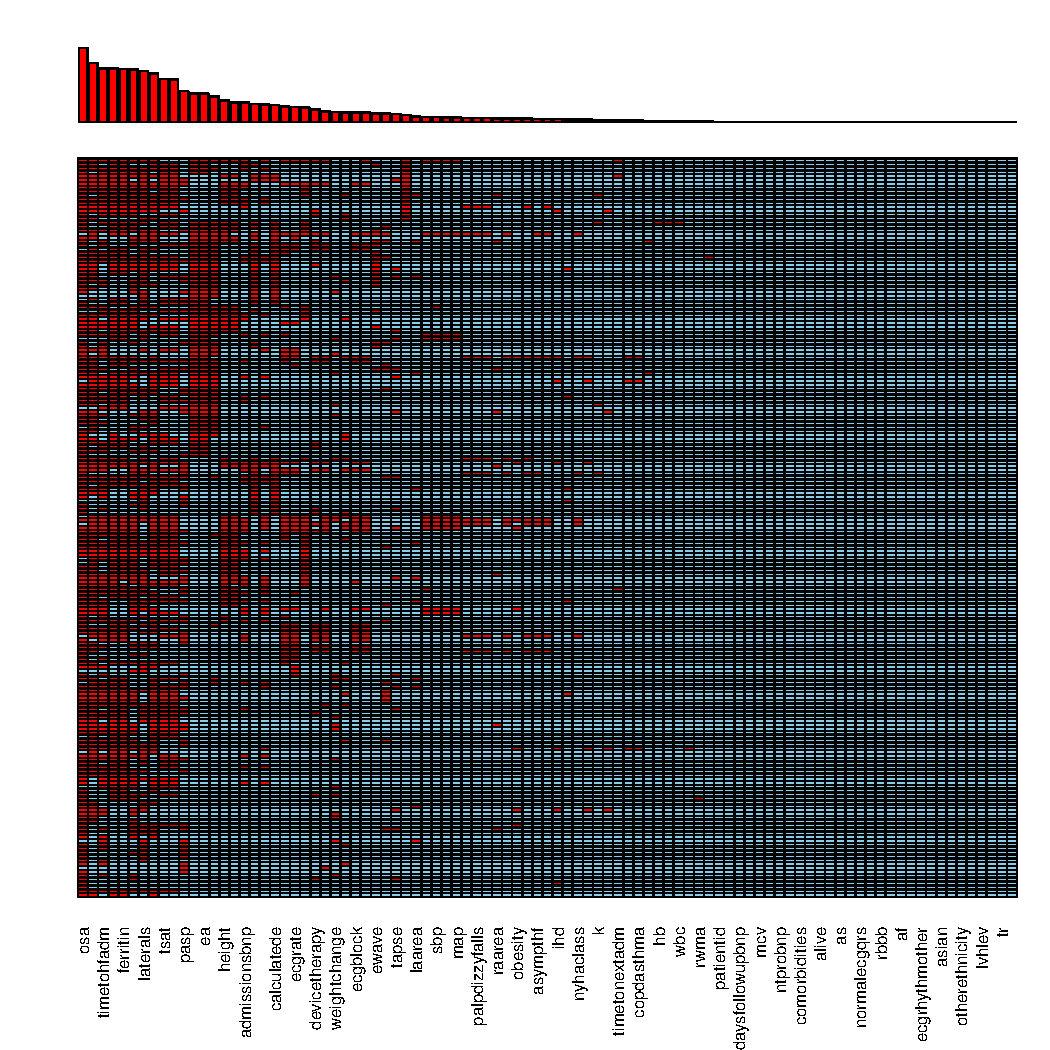
\includegraphics[width=1.1\textwidth]{doc/thesis/images/HFpEF_miss_dist.pdf}
    \caption[Missing values in HFpEF data set]{\textit{Missing values in HFpEF data set. Top:  the amount of missing values in each variable sorted in ascending order. Bottom: plot of the combinations of missing (red) and non-missing (blue) values in the HFpEF data set.}}
    \label{fig:HFpEF_missing}
\end{figure}

\newpage

\begin{figure}[h!]
    \centering
    \hspace*{-1cm}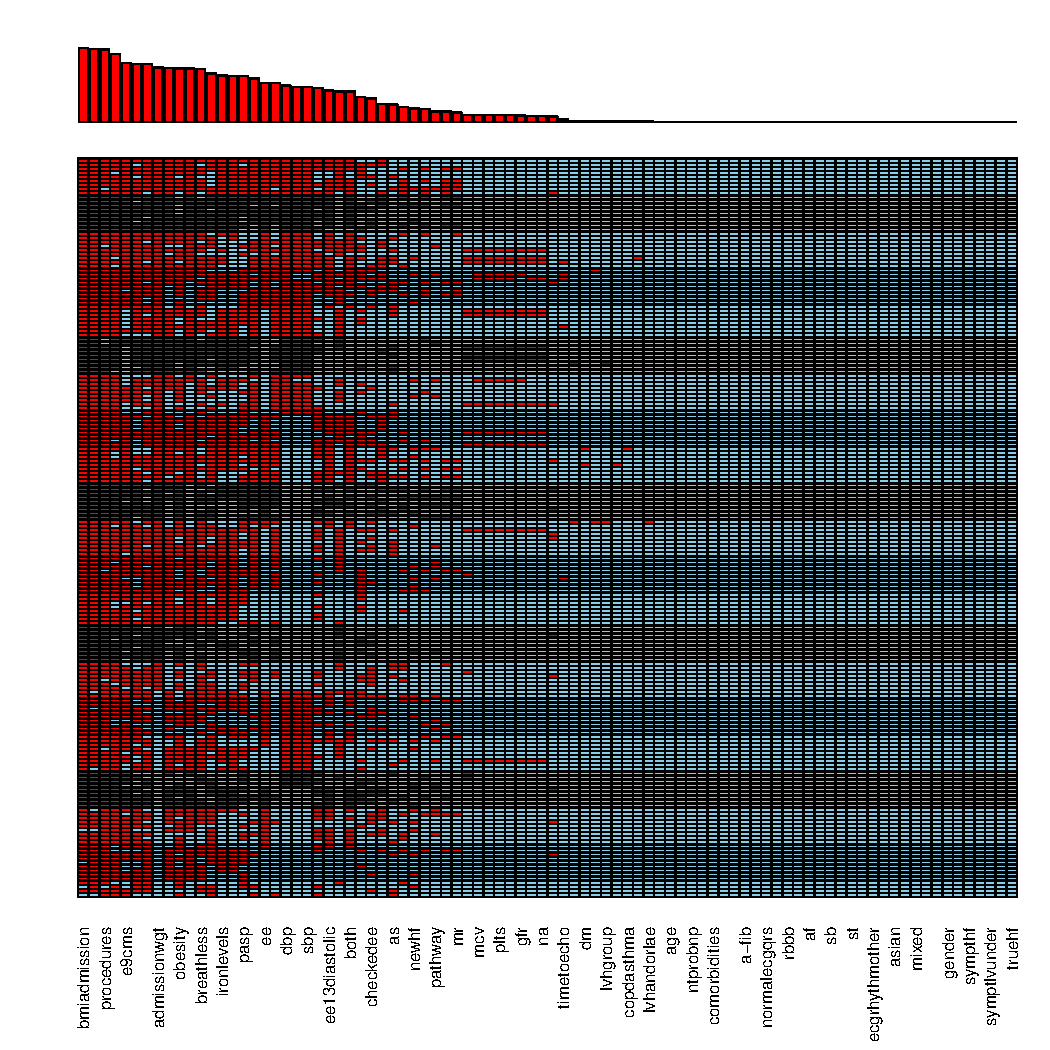
\includegraphics[width=1.1\textwidth]{doc/thesis/images/HFmrEF_miss_dist.pdf}
    \caption[Missing values in HFmrEF data set]{\textit{Missing values in HFmrEF data set. Top:  the amount of missing values in each variable sorted in ascending order. Bottom: plot of the combinations of missing (red) and non-missing (blue) values in the HFmrEF data set.}}
    \label{fig:HFmrEF_missing}
\end{figure}

\newpage

\begin{figure}[h!]
    \centering
    \hspace*{-1cm}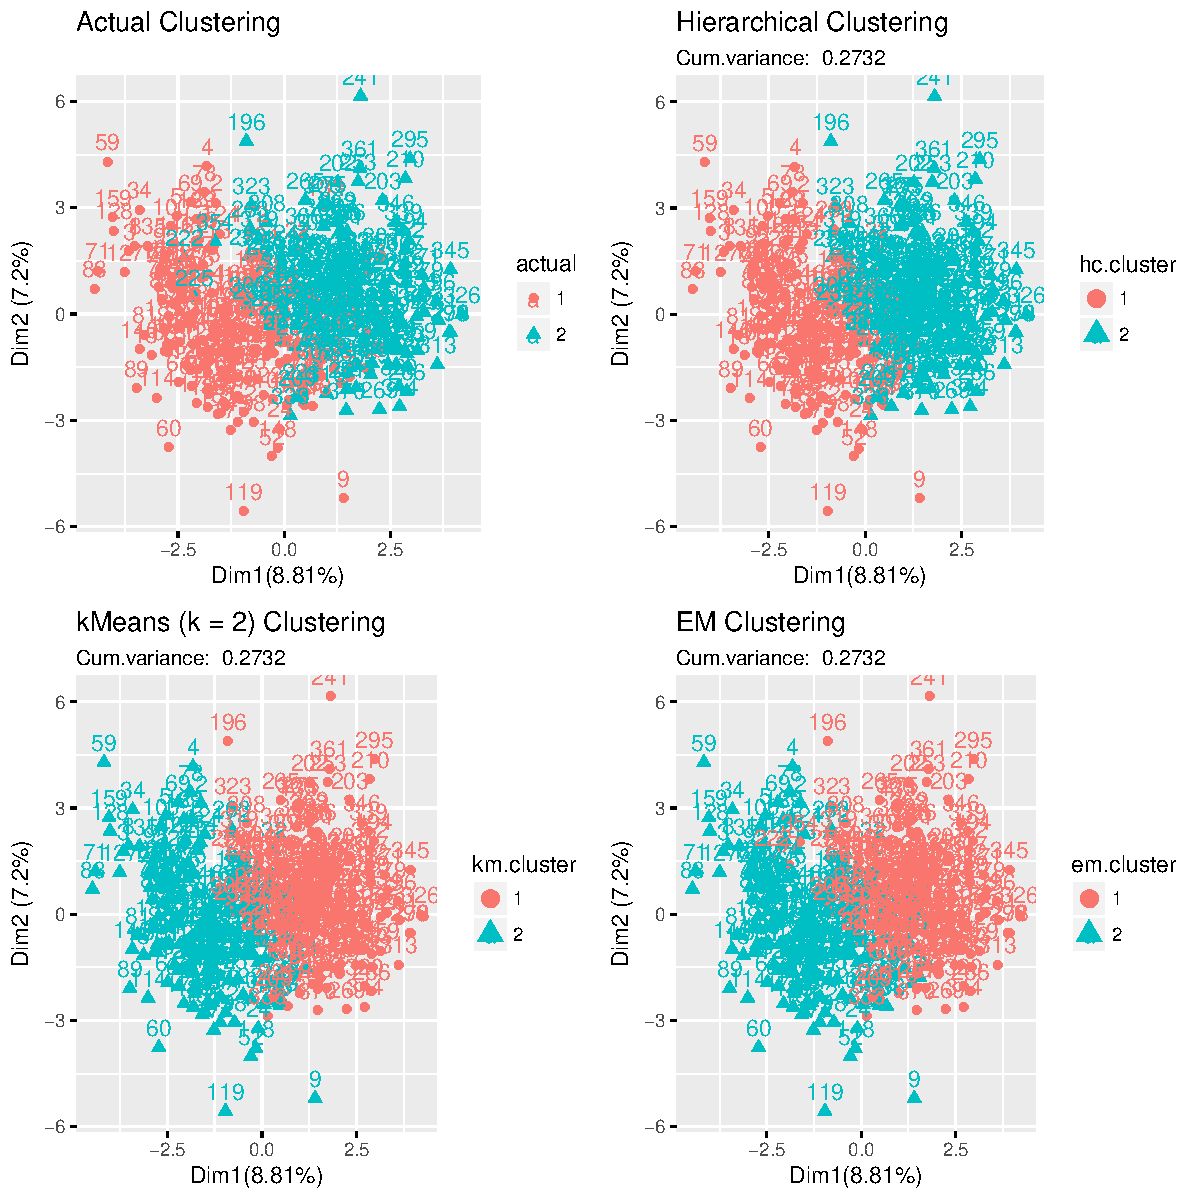
\includegraphics[width=1.1\textwidth]{doc/thesis/images/ClustFull.pdf}
    \caption[Binary clustering problem]{\textit{Results of Binary clustering problem}}
    \label{fig:bi_clust_results}
\end{figure}

\newpage

\begin{figure}[h!]
    \centering
    \hspace*{-1cm}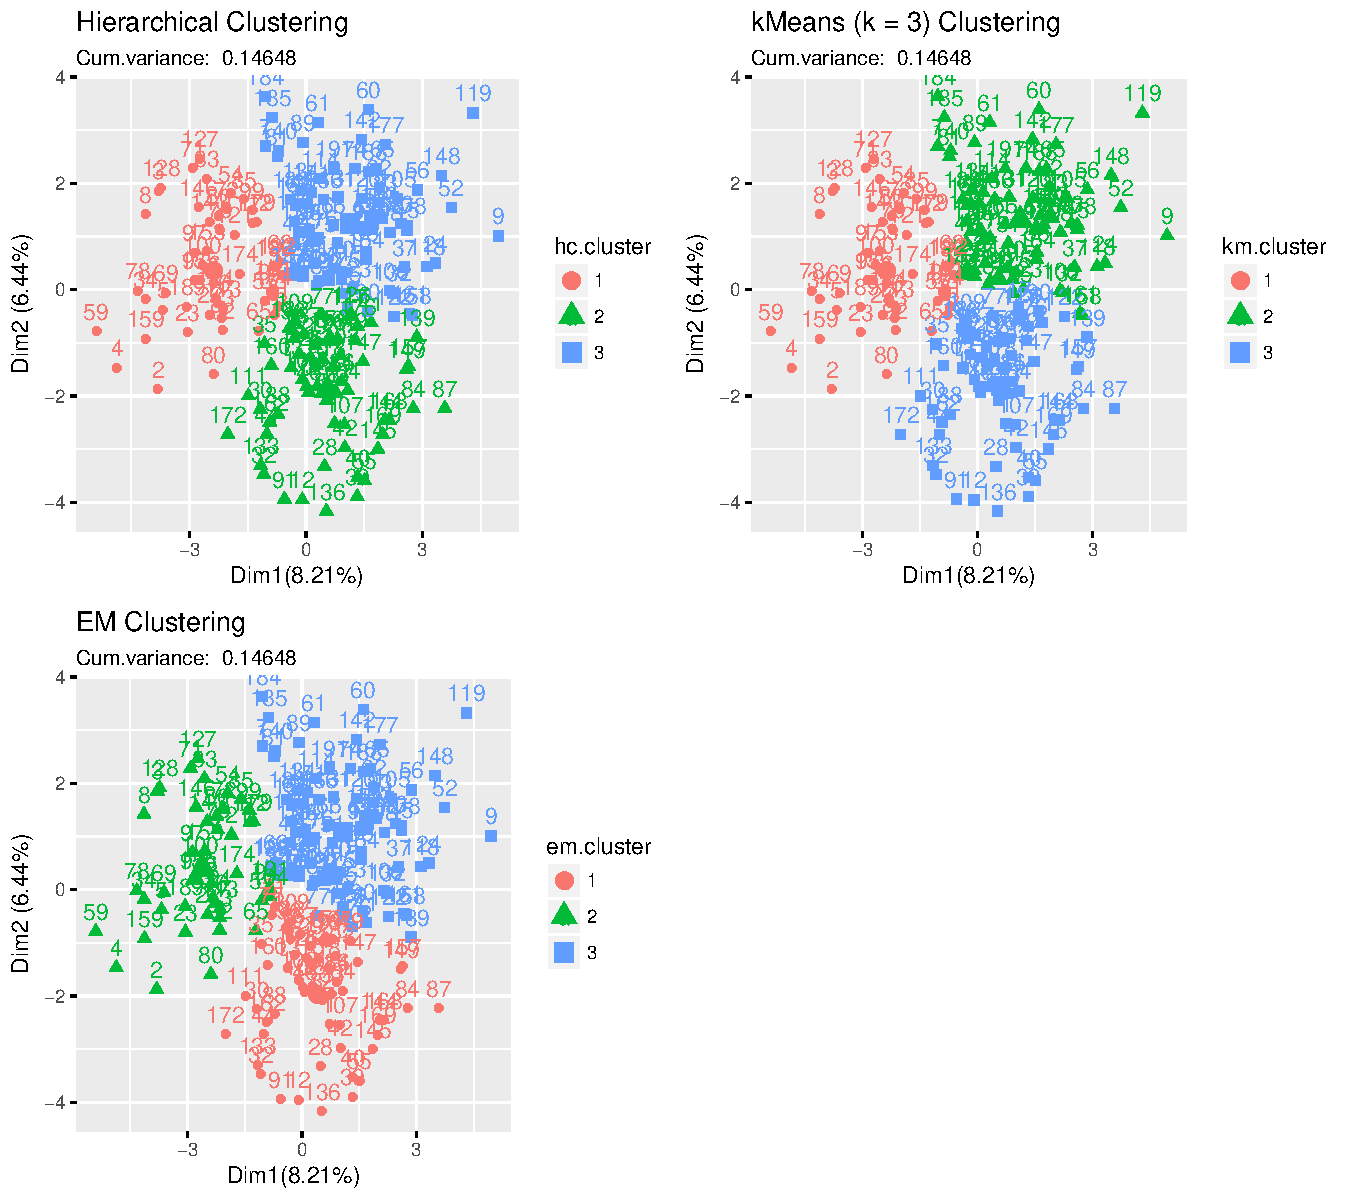
\includegraphics[width=1.1\textwidth]{doc/thesis/images/ClustpPhy.pdf}
    \caption[HFpEF with Post-Diagnosis]{\textit{Clustering results of HFpEF with Post-Diagnosis}}
    \label{fig:clust_results_with_post_p}
\end{figure}

\newpage

\begin{figure}[h!]
    \centering
    \hspace*{-1cm}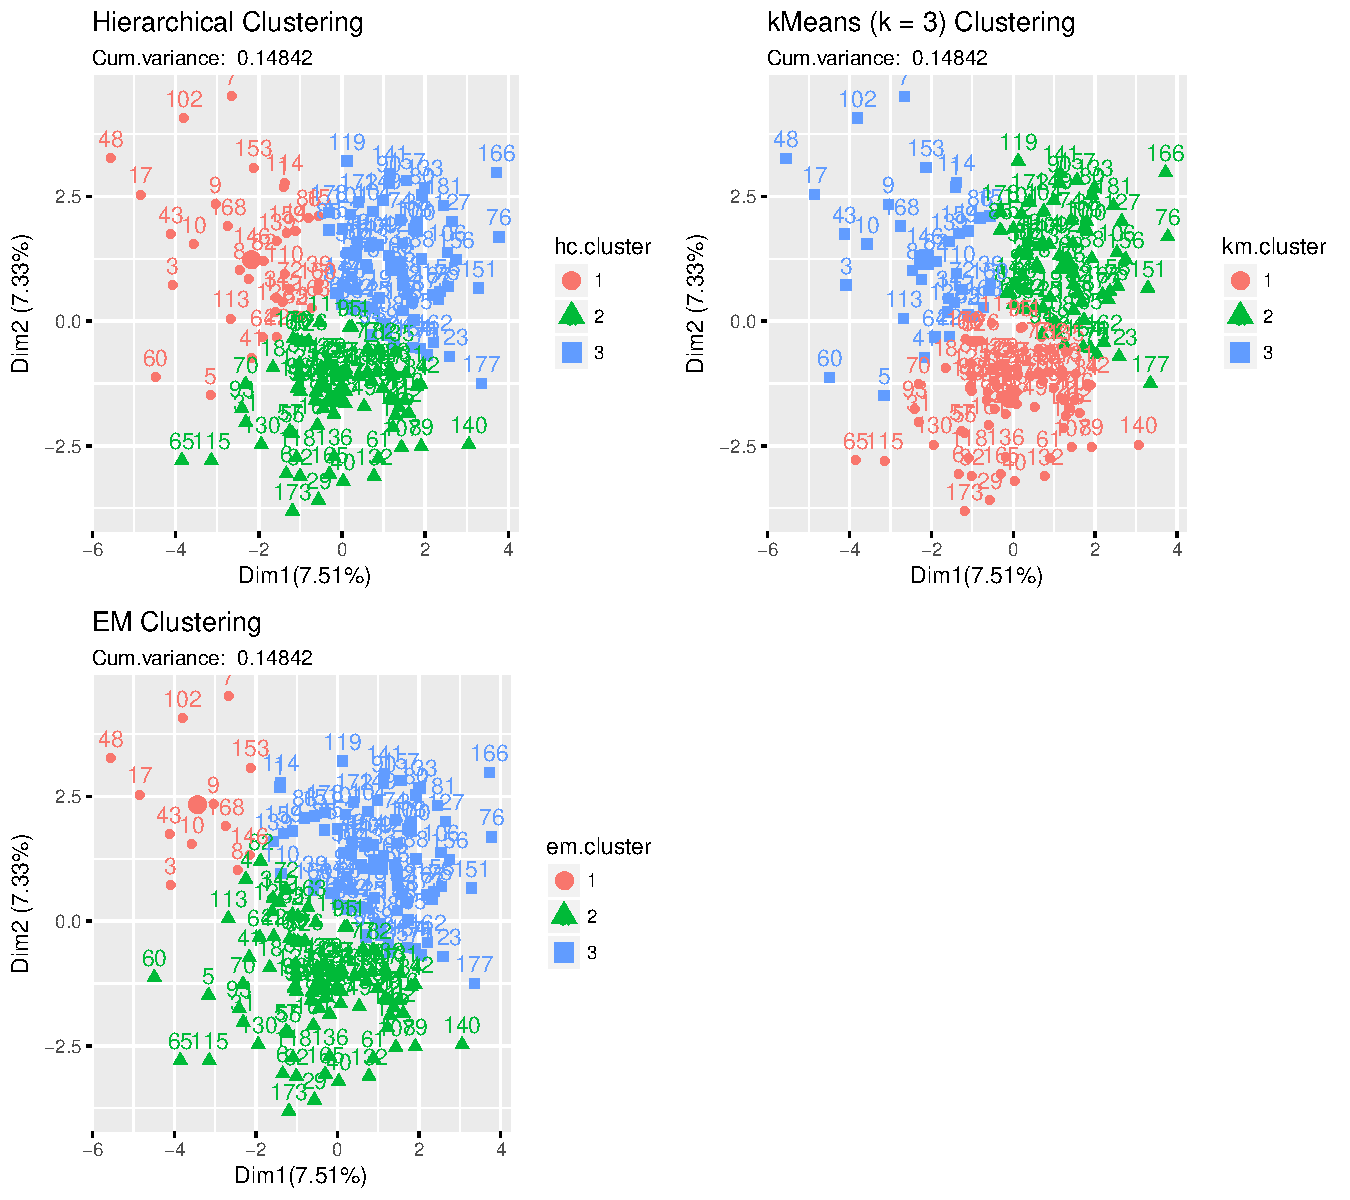
\includegraphics[width=1.1\textwidth]{doc/thesis/images/ClustmrPhy.pdf}
    \caption[HFmrEF with Post-Diagnosis]{\textit{Clustering results of HFmrEF with Post-Diagnosis}}
    \label{fig:clust_results_with_post_mr}
\end{figure}

\newpage

\begin{figure}[h!]
    \centering
    \hspace*{-1cm}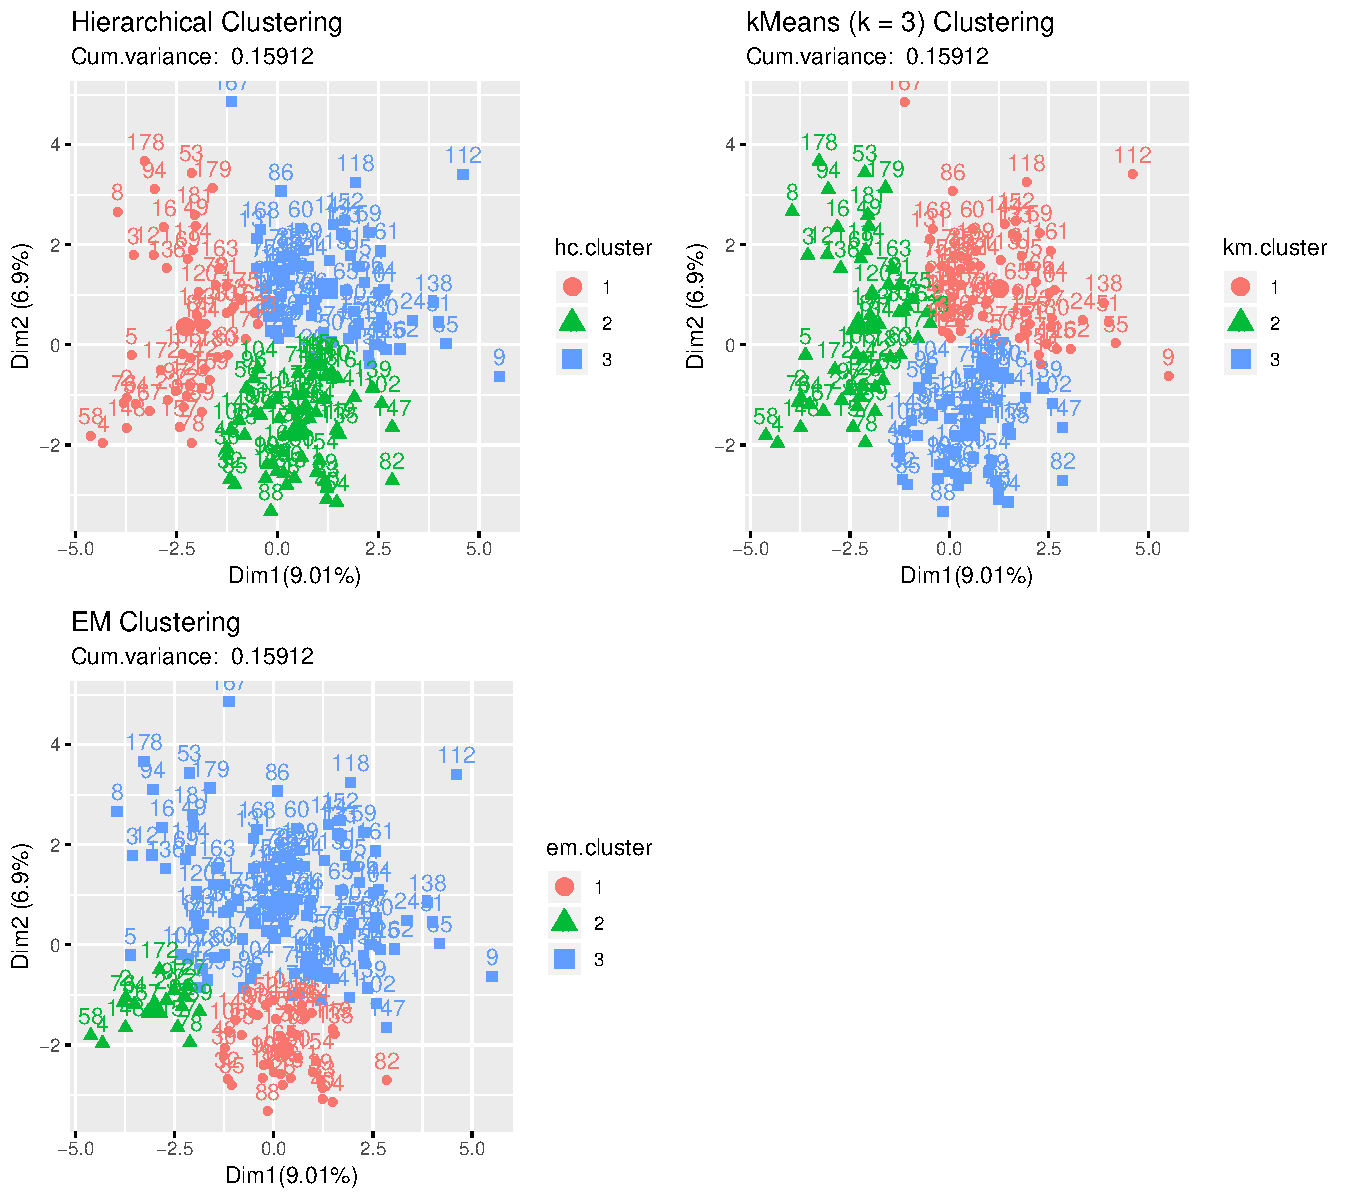
\includegraphics[width=1.1\textwidth]{doc/thesis/images/ClustpNoPhy.pdf}
    \caption[HFpEF without Post-Diagnosis]{\textit{Clustering results of HFpEF \textit{without} Post-Diagnosis}}
    \label{fig:clust_results_without_post_p}
\end{figure}

\newpage

\begin{figure}[h!]
    \centering
    \hspace*{-1cm}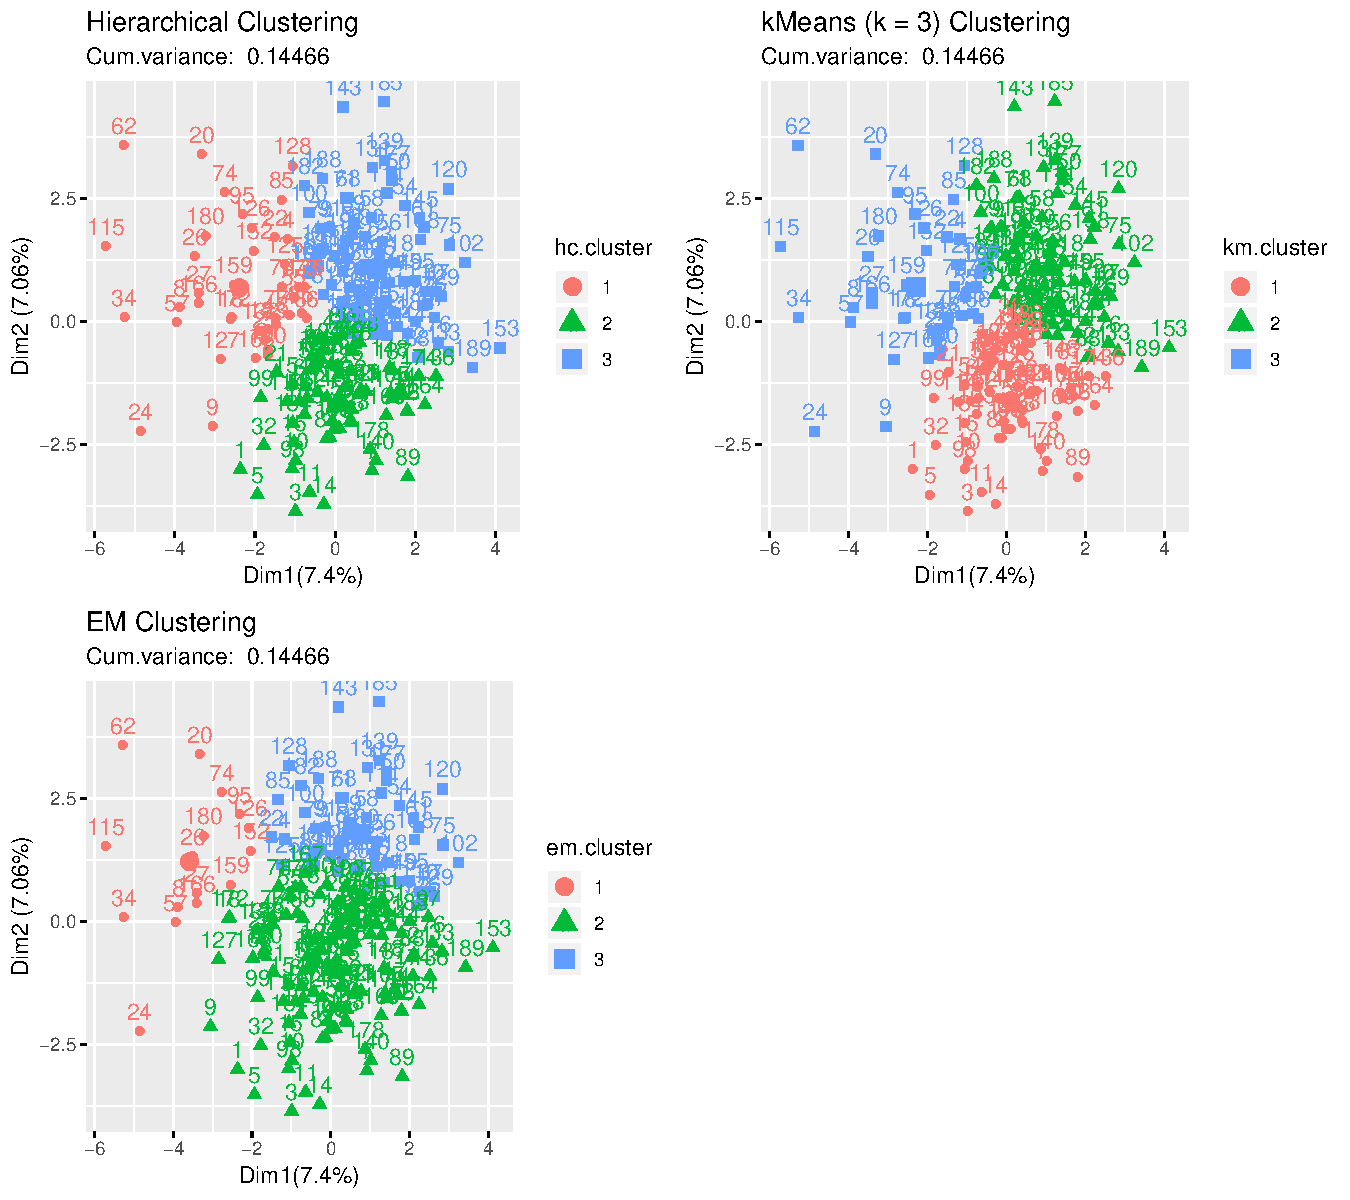
\includegraphics[width=1.1\textwidth]{doc/thesis/images/ClustmrNoPhy.pdf}
    \caption[HFmrEF without Post-Diagnosis]{\textit{Clustering results of HFmrEF \textit{without} Post-Diagnosis}}
    \label{fig:clust_results_without_post_mr}
\end{figure}

\chapter{Source code}
\label{chap:souce_code}

\noindent The following appendix presents all the relevant \texttt{R}-code used in this thesis. We have organized the chapter in accordance with the various steps in the machine learning procedure adopted in this thesis, see Figure (\ref{fig:ML_proc_thesis}). We have tried to comment as much of the source code in order to ensure that an eventual re-examination of the results can be as easy as possible. Inquires about the code can be forwarded to the author on request.

\section{Packages}
\label{sec:pack_code}

\lstinputlisting[language=R]{../../data/data_sets/source/packages.R}

\section{Utilities}
\label{sec:utilities}

\lstinputlisting[language=R]{../../data/data_sets/source/utilities.R}

\section{Descriptive statistics}
\label{sec:app_desc_stat}

\lstinputlisting[language=R]{../../data/data_sets/source/desc_stat.R}

\section{Pre-processing}
\label{sec:pre_proc}

\lstinputlisting[language=R]{../../data/data_sets/source/pre_process.R}
\newpage
\subsection{Consolidation}
\label{sec:consolidation}

\lstinputlisting[language=R]{../../data/data_sets/raw_data/consolidation.R}

\section{Clustering}
\label{sec:clust}

\lstinputlisting[language=R]{../../data/data_sets/source/clustering.R}

\section{Classification}
\label{sec:classifi}

\lstinputlisting[language=R]{../../data/data_sets/source/classification.R}

\end{document}